\documentclass{article}
\usepackage{oconnor}
\usepackage{ wasysym }

%% UPDATE these variables:
\renewcommand{\hwnum}{2}
\title{CSCI 338, Test 02}
\author{Patrick O'Connor (v75j556)}
\collab{n/a}
%%\date{due: 15 January 2021}

\begin{document}

\maketitle

CSCI 338 Computer Science Theory

Test 2 - 70 Minutes

% ============================================
% ============================================
\nextprob{Question 1}
\collab{n/a}
% ============================================
{True or False}
\paragraph{Answer}
\begin{enumerate}
    \item 
    \item 
    \item 
    \item 
\end{enumerate}
% ============================================
% ============================================
\nextprob{Question 2}
\collab{n/a}
% ============================================

\paragraph{Answer}

% ============================================
% ============================================
\nextprob{Question 3}
\collab{n/a}
% ============================================

\paragraph{Answer}


\begin{figure}
    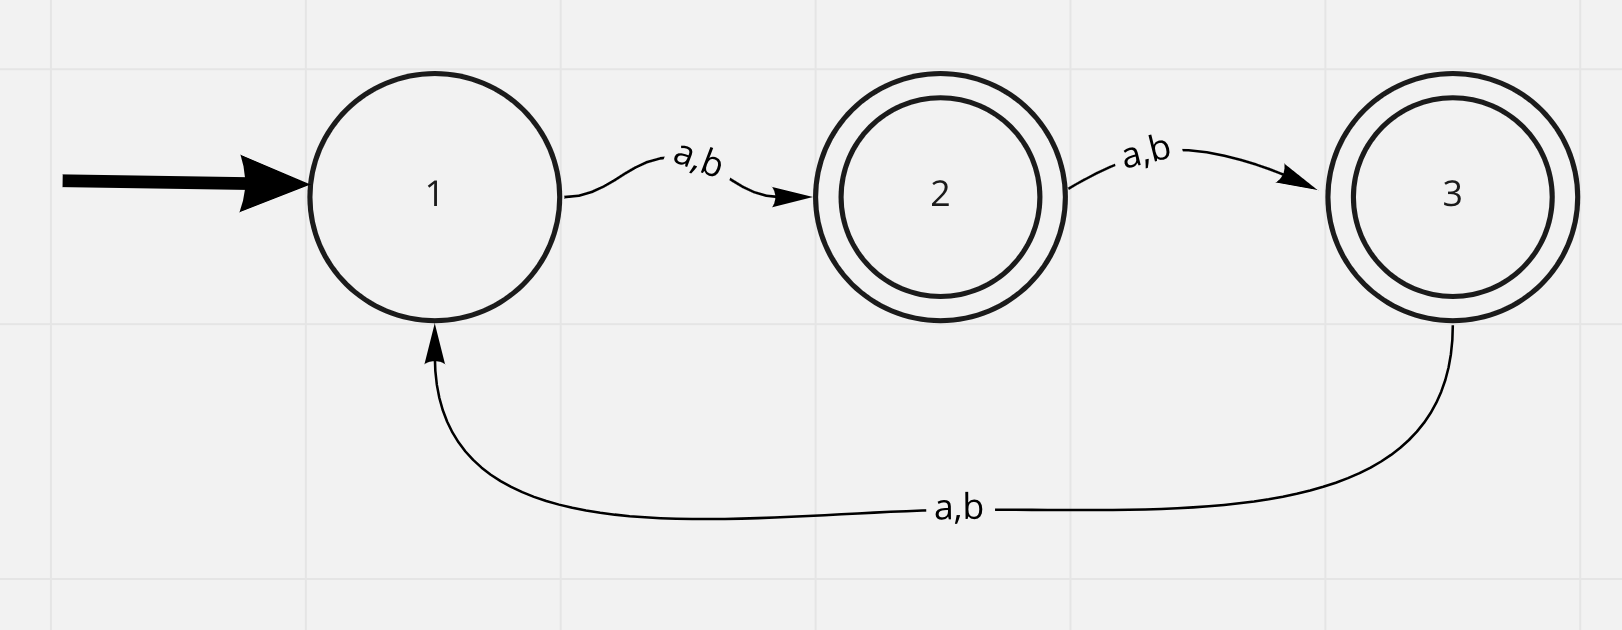
\includegraphics[width=\linewidth]{question03.png}
    \caption{Solution drawn using Miro Board}
    \label{fig:num03}
\end{figure}
Please see figure \ref{fig:num03}


% ============================================
% ============================================
\nextprob{Question 4}
\collab{n/a}
% ============================================

\paragraph{Answer}
\begin{figure}
    \includegraphics[width=\linewidth]{question04.png}
    \caption{Solution hand written}
    \label{fig:num04}
\end{figure}
Please see figure below \ref{fig:num04}

\end{document}

